% Asset ID: FA22MomentumImpulseFoundationsForRestitutionTikZ-002
% Asset type: TikZ diagram
% Topic ID: FA22MomentumImpulseFoundationsForRestitution
% Lesson file: FA22_momentum_impulse_foundations_for_restitution_lesson.md
% Related lesson section: Section 9: Visual Asset Integration
% Source: FM1-Chp1-Momentum.pdf PCLM slide + transcript Newton's third law explanation
% Purpose: Show equal and opposite impulses during a collision.

\documentclass[tikz,border=8pt]{standalone}
\usepackage{amsmath}
\usepackage{xcolor}
\usetikzlibrary{arrows.meta, positioning, calc, decorations.pathreplacing}
\definecolor{Canvas}{HTML}{FAF9F6}
\definecolor{Panel}{HTML}{FFFFF0}
\definecolor{Line}{HTML}{E5E5EA}
\definecolor{Accent}{HTML}{C5A059}
\definecolor{SoftPink}{HTML}{FBEFEF}
\definecolor{Text}{HTML}{2C2C2E}
\definecolor{Muted}{HTML}{6B6B70}
\begin{document}
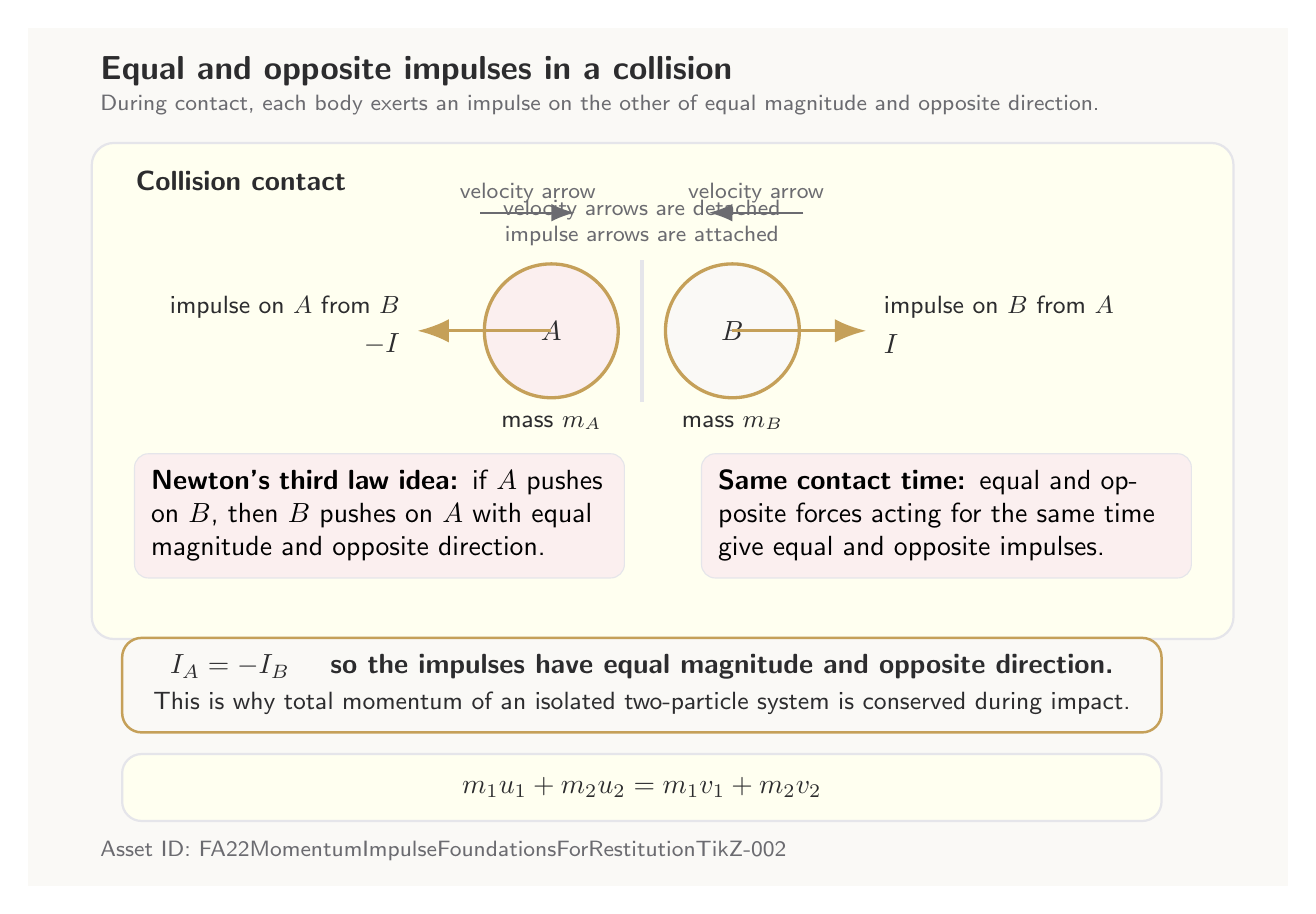
\begin{tikzpicture}[font=\sffamily,>=Latex,impulse/.style={-{Latex[length=4mm]}, very thick, draw=Accent},velocity/.style={-{Latex[length=3mm]}, thick, draw=Muted},panel/.style={draw=Line, fill=Panel, rounded corners=8pt, line width=0.8pt},note/.style={draw=Line, fill=SoftPink, rounded corners=5pt, inner sep=6pt},titletext/.style={text=Text, font=\sffamily\bfseries\large},labeltext/.style={text=Text, font=\sffamily\small},eqtext/.style={text=Text, font=\sffamily\bfseries},smallmuted/.style={text=Muted, font=\sffamily\footnotesize}]
\fill[Canvas] (-0.8,-5.7) rectangle (15.2,5.2);
\node[titletext, anchor=west] at (0,4.65) {Equal and opposite impulses in a collision};
\node[smallmuted, anchor=west] at (0,4.22) {During contact, each body exerts an impulse on the other of equal magnitude and opposite direction.};
\node[panel, minimum width=14.5cm, minimum height=6.3cm, anchor=north west] at (0,3.75) {};
\node[eqtext, anchor=west] at (0.45,3.25) {Collision contact};
\filldraw[fill=SoftPink, draw=Accent, line width=1.2pt] (5.85,1.35) circle (0.85);
\filldraw[fill=Canvas, draw=Accent, line width=1.2pt] (8.15,1.35) circle (0.85);
\node[eqtext] at (5.85,1.35) {$A$}; \node[eqtext] at (8.15,1.35) {$B$};
\node[labeltext] at (5.85,0.18) {mass $m_A$}; \node[labeltext] at (8.15,0.18) {mass $m_B$};
\draw[Line, line width=1.2pt] (7.0,0.45) -- (7.0,2.25);
\draw[impulse] (5.85,1.35) -- (4.15,1.35);
\node[labeltext, anchor=east] at (4.05,1.65) {impulse on $A$ from $B$};
\node[eqtext, anchor=east] at (4.05,1.18) {$-I$};
\draw[impulse] (8.15,1.35) -- (9.85,1.35);
\node[labeltext, anchor=west] at (9.95,1.65) {impulse on $B$ from $A$};
\node[eqtext, anchor=west] at (9.95,1.18) {$I$};
\draw[velocity] (4.95,2.85) -- (6.15,2.85); \node[smallmuted] at (5.55,3.1) {velocity arrow};
\draw[velocity] (9.05,2.85) -- (7.85,2.85); \node[smallmuted] at (8.45,3.1) {velocity arrow};
\node[smallmuted, align=center] at (7.0,2.72) {velocity arrows are detached\\impulse arrows are attached};
\node[note, text width=5.8cm, anchor=west] at (0.55,-1.0) {\textbf{Newton's third law idea:} if $A$ pushes on $B$, then $B$ pushes on $A$ with equal magnitude and opposite direction.};
\node[note, text width=5.8cm, anchor=west] at (7.75,-1.0) {\textbf{Same contact time:} equal and opposite forces acting for the same time give equal and opposite impulses.};
\node[draw=Accent, fill=Canvas, rounded corners=7pt, line width=0.9pt, minimum width=13.2cm, minimum height=1.2cm] at (7,-3.15) {};
\node[eqtext] at (7,-2.92) {$I_A=-I_B$ \quad so the impulses have equal magnitude and opposite direction.};
\node[labeltext] at (7,-3.38) {This is why total momentum of an isolated two-particle system is conserved during impact.};
\node[draw=Line, fill=Panel, rounded corners=7pt, line width=0.8pt, minimum width=13.2cm, minimum height=0.85cm] at (7,-4.45) {};
\node[eqtext] at (7,-4.45) {$m_1u_1+m_2u_2=m_1v_1+m_2v_2$};
\node[smallmuted, anchor=west] at (0,-5.25) {Asset ID: FA22MomentumImpulseFoundationsForRestitutionTikZ-002};
\end{tikzpicture}
\end{document}
